% !TEX root=/home/tavant/these/manuscript/src/manuscript.tex


\section{Characteristics of the azimuthal instability}
  \label{sec-Ztheta-instability}

  We have observed in the previous section that the radial loss model did not modify significantly the plasma characteristics (densities, axial electric field), but it had a significant impact on the electron cross-field transport.
  Since the simulations are collisionless, the origin of the variation of the electron axial mobility comes from the azimuthal instability, which amplitude decreases with the radial losses as seen in \cref{fig-boeuf-instability}.
  In this section, we investigate the possible mechanism responsible of the evolution of the oscillation characteristics.
  Several phenomena can have an impact, direct or indirect, on the azimuthal instability\string:
  \begin{enumerate}
    \item The radial loss algorithm used could induce numerical noise which affect the instability,
    \item The electron temperature is decreased\string; if the amplitude of the instability saturates due to ion-wave trapping, then the amplitude would be lower,has developed in \cref{eq-iontropempl},
    \item The growth rate is proportional to the azimuthal electron drift velocity, as seen in \cref{eq-MIAW}. If the growth rate is affected, then the wave amplitude at steady state could be reduced,
    \item The radial losses  could directly reduce the amplitude of the density oscillation.
  \end{enumerate}

  Using the results of the \ac{2D} \ac{PIC} simulation, we will discuss the four points in the next sections.
  



\subsection{Overview of the azimuthal instability} \label{subsec-azi_insta_Ztheta}
  
  \begin{figure}[hbt]
    \centering
    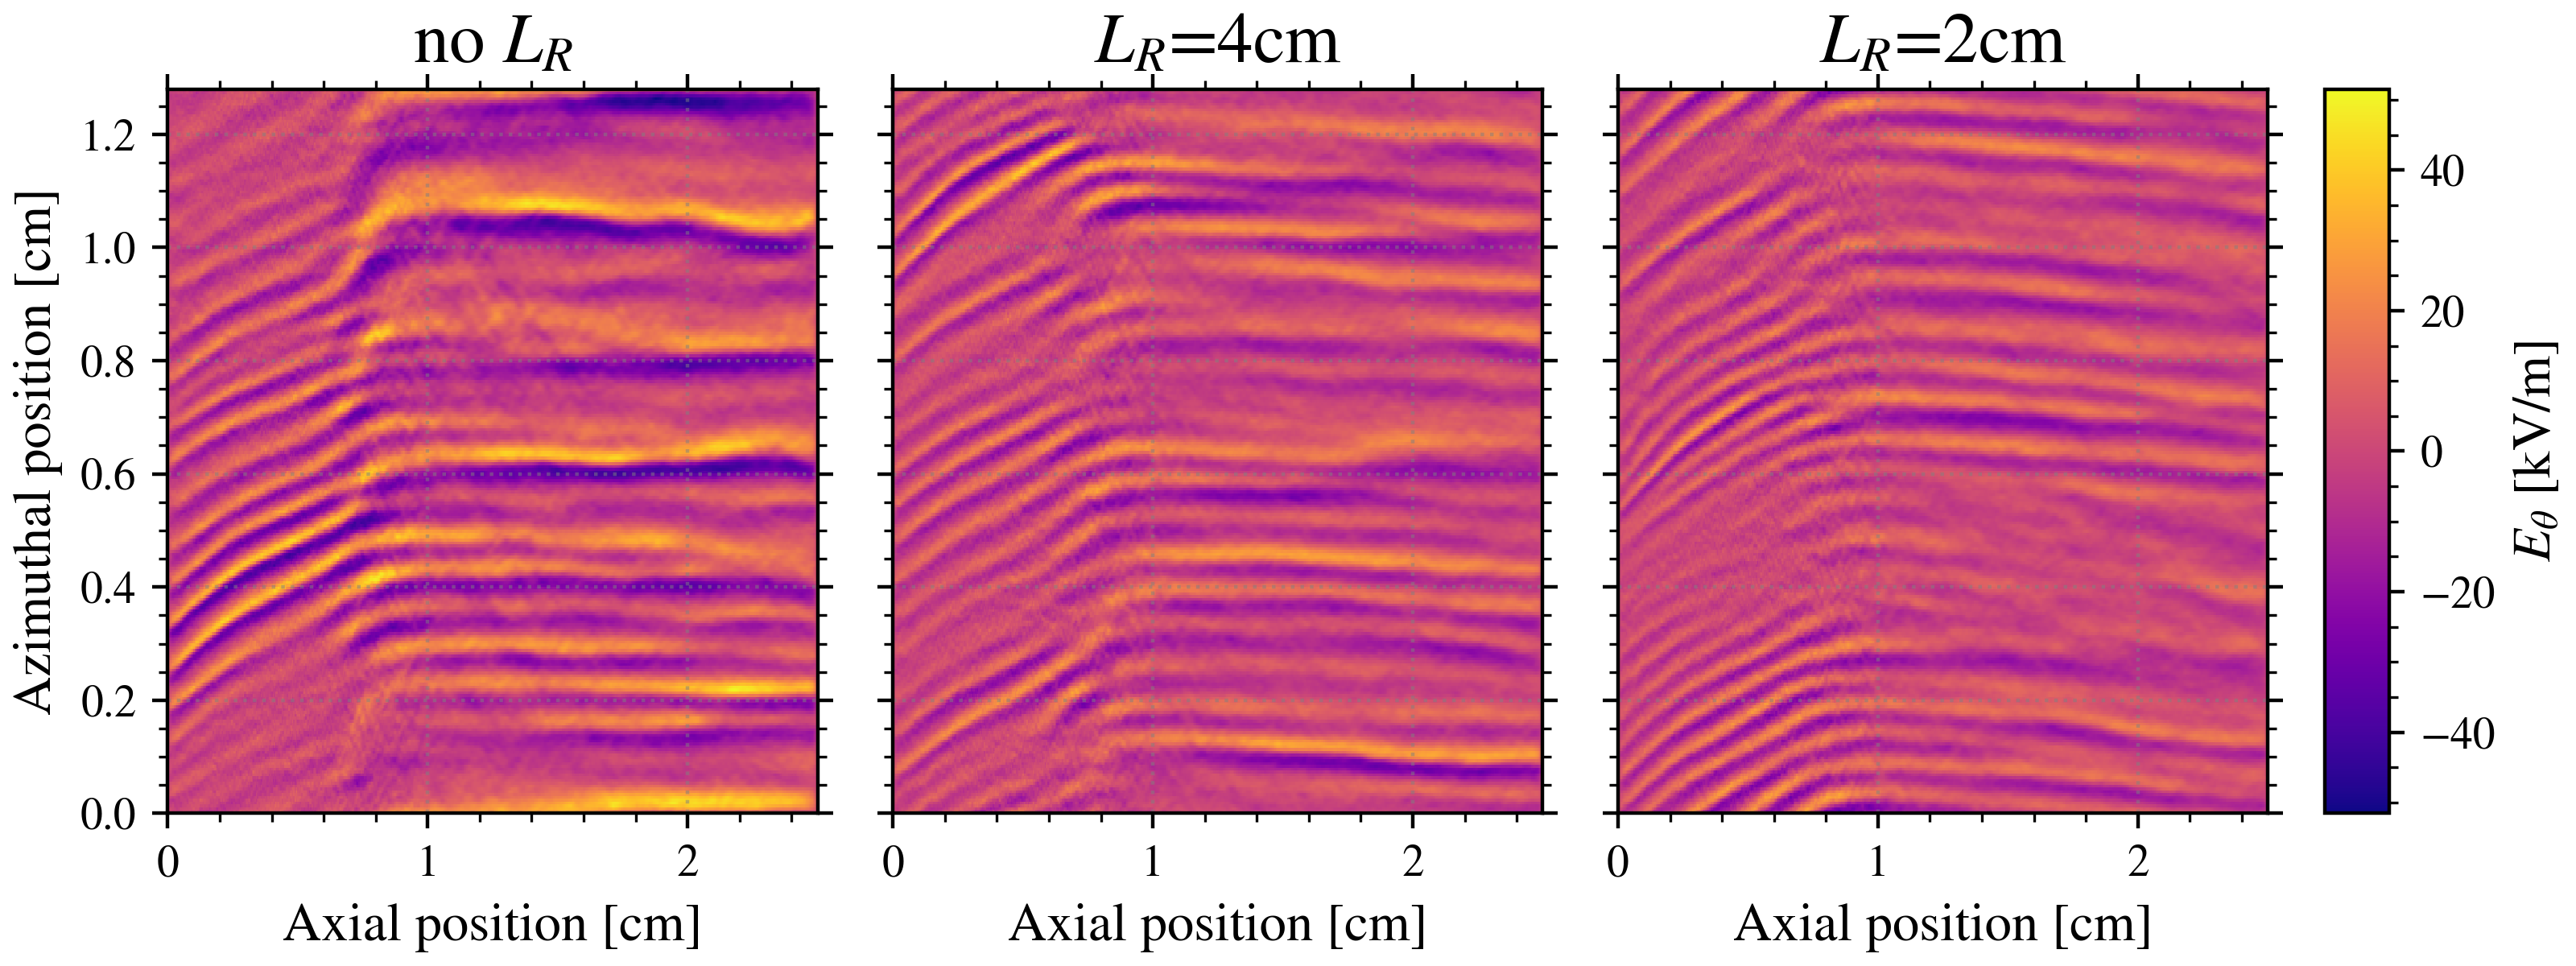
\includegraphics[width=\textwidth]{Boeuf_Ex_snapshot}
    \caption{Axial and azimuthal distribution of the azimuthal electric field $E_{\theta}$  obtained at $t=10 \,\micro\second$ for the three cases using the model of Boeuf. The same color limits are used for each figure.}
    \label{fig-snapshots}
  \end{figure}
  We recall that three cases have been simulated\string: the nominal case without radial losses and two other cases with the radial losses modeled with $L_R=2\,\centi\meter$ or $L_R=4\,\centi\meter$.
  \Cref{fig-snapshots} shows the azimuthal electric field at the end of the simulation for the three cases.
  The azimuthal instability is present in all the simulation domain.
  We note that the radial losses do not induce unphysical instabilities, such as observe in \cref{sec-reinjectionnoise} with the modeling of the axial convection in radial-azimuthal simulations.
  Therefore, we believe that there is no numerical noise or artifacts that affects the instability.
  This conclusion is confirmed by the spectra analysis of \cref{subsec-fft_losses}.
  From the characteristics of the instability seen in \cref{fig-snapshots}, two zones can be identified\string:
  \begin{itemize}
    \item The upstream region, $z < 8 \,\milli\meter$, where the instability presents a short wavelength, and is oblique.
    \item The downstream region, $z > 1\,\centi\meter$, where the wavelength of the instability is larger and is almost perfectly azimuthal.
  \end{itemize}
  The radial losses seem to reduce the wavelength of the instability in both regions, but the main impact is in the downstream region.


  We have seen in \cref{ch-5} that the instability wavelength is of the order of the Debye length $\lde$ and its frequency is of the order of the ion plasma frequency $\opi$.
  In contrast with \cref{ch-5}, the two parameters now vary in the simulation domain.
  \Cref{fig-wpi_Lde} shows the axial evolution of the ion plasma frequency and the Debye length for the three cases.
  The Debye length is calculated using the azimuthal temperature $\Te_{\theta}$.
  

  \begin{figure}[hbt]
    \centering
    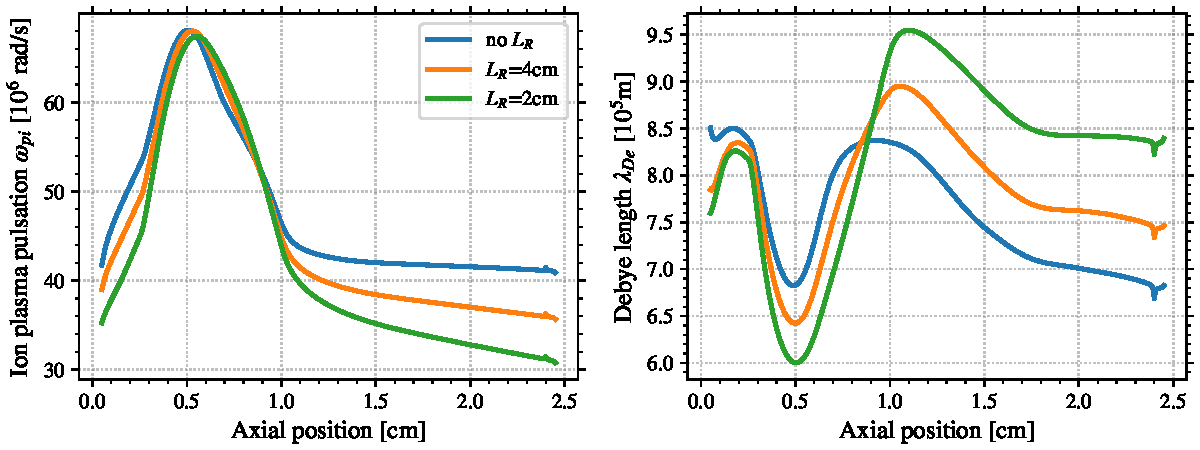
\includegraphics[width=\textwidth]{Boeuf_opi_Lde}
    \caption{Axial evolution of (left) the ion plasma frequency $\opi$ and (right) the Debye length $\lde$ for the three cases averaged  azimuthally and in time between $t=6\,\micro\second$ and $t=10\,\micro\second$.}
    \label{fig-wpi_Lde}
  \end{figure}

  We see in \cref{fig-wpi_Lde} that $\opi$ reaches a maximum at $z=0.5\,\centi\meter$, and decreases by almost a factor of two towards both the anode and the cathode.
  We observe that $\opi$ is not significantly affected by the radial losses in the upstream region, but decreases with the increase of the losses in the downstream region.
  On the other hand, the Debye length $\lde$ presents a more complex behavior, as it reaches a local minima at $z=0.5\,\centi\meter$ and a local maxima at $z\simeq 1\,\centi\meter$.
  The amplitude of the evolution of $\lde$ is smaller compared to $\opi$, as it changes in the axial direction by approximately $20\%$ without the radial, and up to $40\%$ with $L_R=2\,\centi\meter$.
  In addition, we see in \cref{fig-wpi_Lde} that the radial losses change $\lde$ in both regions, but not with the same trend.
  In the upstream region, the radial losses decrease $\lde$, while they increase $\lde$ in the downstream region.


\subsection{Ion-wave trapping saturation } \label{subsec-boeuf_iontrapping}

  The test-case used here and proposed by \citet{boeuf2018} allows the simulation to reach a steady-state.
  The authors state that the amplitude of the instability is consistent with an ion-wave trapping saturation.
  Therefore, we use the criterion developed in \cref{subsec-temp} and given by \cref{eq-criteriaIT} to determine whether or not the modification of the wave amplitude is related to the ion-wave trapping.
  We recall the criterion used between the thermal and the wave energy densities
  \begin{equation} 
    432 \epsilon_{\rm wave} = \epsilon_{\rm th},
  \end{equation}
  with $\epsilon_{\rm th} = \frac{3}{2} e n_e \Te$ and $\epsilon_{\rm wave} = \frac{\epsilon_0}{2} \stdE^2$.
  \Cref{fig-ionwavetrapping_axial} shows the axial profile of the ration between $432 \epsilon_{\rm wave}$ and $\epsilon_{\rm th}$,  averaged  azimuthally and in time between $t=6\,\micro\second$ and $t=10\,\micro\second$ for the three cases of radial losses.

  \begin{figure}[hbt]
    \centering
    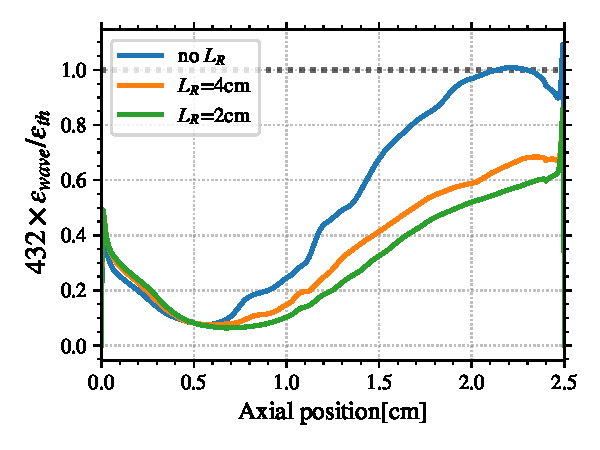
\includegraphics[width=\defaultwidth]{Boeuf_Axial_IonTrapping_criter}
    \caption{Axial evolution of the ration between $432 \epsilon_{\rm wave}$ and $\epsilon_{\rm th}$ to characterize the ion-wave trapping, averaged azimuthally and between $t=6\,\micro\second$ and $t=10\,\micro\second$ for the three radial losses cases. }
    \label{fig-ionwavetrapping_axial}
  \end{figure}

  We see that the results observed for the case without radial losses do reach the saturation criteria, but only close to the cathode for $z > 2\,\centi\meter$.
  Nevertheless, for both cases with the radial losses modeled, the amplitude on the wave is smaller.
  Hence, it seems that the wave amplitude is reduced by the radial losses such that the ion-wave trapping is not the dominant saturation mechanism anymore.


  % \begin{figure}[hbt]
  %   \centering
  %   \begin{tabular}{@{} cc}
  %     \subfigure{Boeuf_iontrapping_Lr4}{a}{20,65} & 
  %     \subfigure{Boeuf_iontrapping_Lr2}{b}{20,65} \\
  %   \end{tabular}
  %   \caption{Temporal evolution of the ion-wave trapping criterion for the test-case of Boeuf with ({\bf a}) $L_R=4\,\centi\meter$, and ({\bf b}) $L_R=2\,\centi\meter$  at three positions\string: $z=0.25\,\centi\meter$, in the upstream region; $z=1.5\,\centi\meter$, and $z=2.3\,\centi\meter$, in the downstream region.}
  %   \label{fig-ion-trap_temp_Lr}
  % \end{figure}

  % \begin{figure}[hbt]
  %   \centering
  %   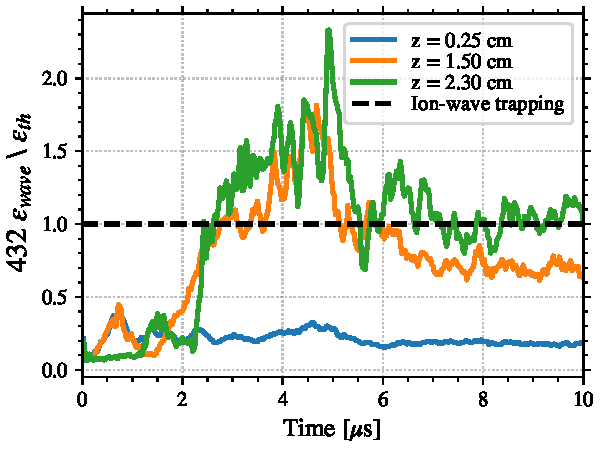
\includegraphics[width=\defaultwidth]{Boeuf_iontrapping_noLr}
  %   \caption{Temporal evolution of the ion-wave trapping criteria for the test-case of Boeuf without radial losses at three positions\string: $z=0.25\,\centi\meter$, in the upstream region; $z=1.5\,\centi\meter$, and $z=2.3\,\centi\meter$, in the downstream region.}
  %   \label{fig-ion-trap_temp_noLr}
  % \end{figure}

\subsection{Electron azimuthal drift velocity} \label{subsec-drift}

  We showed in \cref{ch-5} that the instability growth rate is proportional to the electron azimuthal drift.
  In the radial-azimuthal simulation, the drift was only due to the $\vect{E} \times \vect{B}$ drift
  \begin{equation} \label{eq-exbdrift}
    u_{E \times B} = - \frac{E_z}{B_r}
  \end{equation}
  However, we saw in \cref{fig-boeuf_axialtwo} that the electron density presents a large axial gradient.
  Therefore, the diamagnetic drift
  $$u_{\rm Dia}=\frac{\nabla_z (n_e {\rm T}_{e,z})}{n_e B_r}$$
  can also affect the electron drift velocity.
  \Cref{fig-Jetheta_sum} shows the axial profile of the azimuthal electron mean velocity $u_{e, \theta}$ at steady-state ($t = 14\,\micro\second$) for the case without the radial losses modeled.

 
  \begin{figure}[hbt]
    \centering
    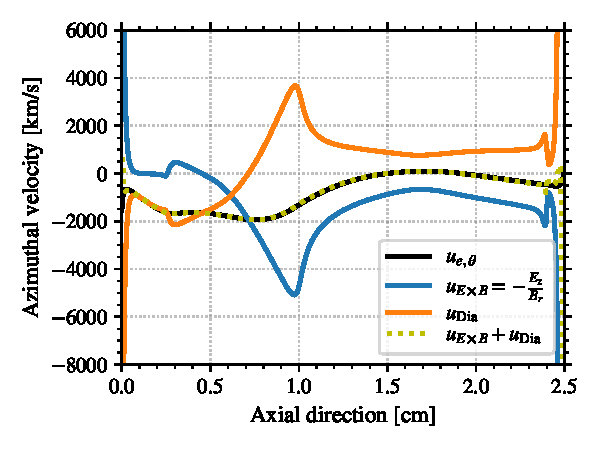
\includegraphics[width=\defaultwidth]{Boeuf_Je_x_axial_one}
    \caption{Axial profile of (black solid line) the electron azimuthal velocity measured in the simulation, (blue solid line) the $\vect{E} \times \vect{B}$ drift velocity, (solid orange line) the diamagnetic velocity, and (dashed line) the sum of the $\vect{E} \times \vect{B}$ and diamagnetic velocities averaged azimuthally and between $t=6\,\micro\second$ and $t=10\,\micro\second$ for the case without radial losses.}
    \label{fig-Jetheta_sum}
  \end{figure}
  
  We can see that the $E \times B$ drift is not the only contribution to the electron azimuthal velocity, in contrast to the radial-azimuthal simulations.
  Instead, we have 
  $$ u_{e, \theta} =   u_{E \times B} + u_{\rm Dia}$$
  everywhere in the simulation domain.
  We see that $u_{\rm Dia}$ is of the same order of magnitude as $u_{E \times B}$, but of opposite sign downstream.
  \Cref{fig-Jetheta} shows the values of $ u_{e, \theta},   u_{E \times B}$, and $u_{\rm Dia}$ for the three cases.
  We can see that the magnitude of $u_{e, \theta} $ decreases when the radial losses are present.
  However, both the amplitude of $u_{\rm Dia}$ and $u_{E \times B}$ decreases.

   
  \begin{figure}[hbt]
    \centering
    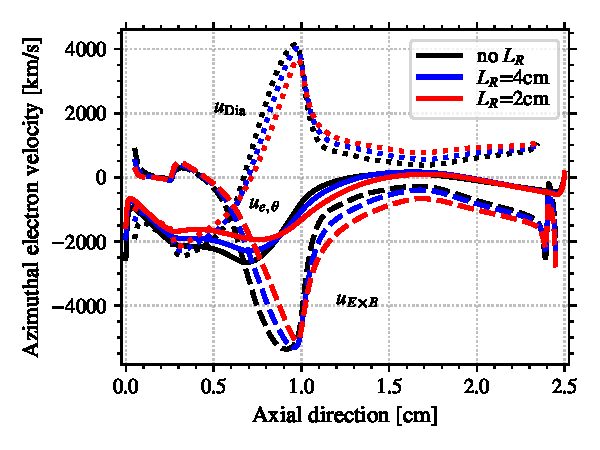
\includegraphics[width=\defaultwidth]{Boeuf_Je_x_axial}
    \caption{Axial profile of the electron azimuthal velocity, the $\vect{E} \times \vect{B}$ drift velocity and the diamagnetic velocity averaged azimuthally and between $t=6\,\micro\second$ and $t=10\,\micro\second$ for the three different radial models for the simulation test-case of Boeuf. The sheaths (close to the axial boundaries) are removed from the figure for clarity purpose.}
    \label{fig-Jetheta}
  \end{figure}

  Despite seeing previously in \cref{sec-Zthetaresults} that the radial losses do not modify significantly the axial electric field and the electron density, the electron azimuthal drift velocity does decrease with the radial losses. 
  At the maximum, the difference represents a 20\% variation, but in average the difference is below 10\%.
  Therefore, the hypothesis of decreased growth rate to explain the reduction of the amplitude of the wave is plausible.

\FloatBarrier


\subsection{Characteristics of the radial losses}

  The last hypothesis on the reduction of the wave amplitude is the direct impact of the radial losses.
  We recall that the electron flux equals the ion flux at each time step\string:
  \begin{equation} \label{eq-fluxequality}
    \Gamma_{R, e} = \Gamma_{R, i}.
  \end{equation}
  The ion flux to the wall is a thermal flux
  \[ \Gamma_{R, i} \propto \bar{v}_{i, r} \]
  with $\bar{v}_{i, r}$ proportional to the radial thermal velocity. 
  However, we have seen that the radial temperature of the particles is constant.
  Assuming the ions distributed uniformly along the radial direction, the particle flux to the wall is proportional to the particle density
  \begin{equation} \label{eq-Rlosses}
    \Gamma_R \propto n_i.
  \end{equation}
  Hence, the particle losses presents the azimuthal fluctuation of the wave
  \[ \Gamma_R(\theta) = \Gamma_0 + \delta \Gamma_R(\theta) \propto (n_{i,0} + \delta_{n_i})  \bar{v}_{i, r} , \]
  with $\Gamma_0$ the mean particle loss, and $ \delta \Gamma_R(\theta)$ the fluctuation of the losses due to the wave.
  \Cref{fig-rfluxs} shows the azimuthal-axial distribution of (left) the radial flux measured in the \ac{PIC} simulation, and (right) the electron density, at $t=10\,\micro\second$ for the case $L_R=2\,\centi\meter$.
  We suppose the quasi-neutrality, hence $n_i = n_e$.

  \begin{figure}[hbtp]
    \centering
    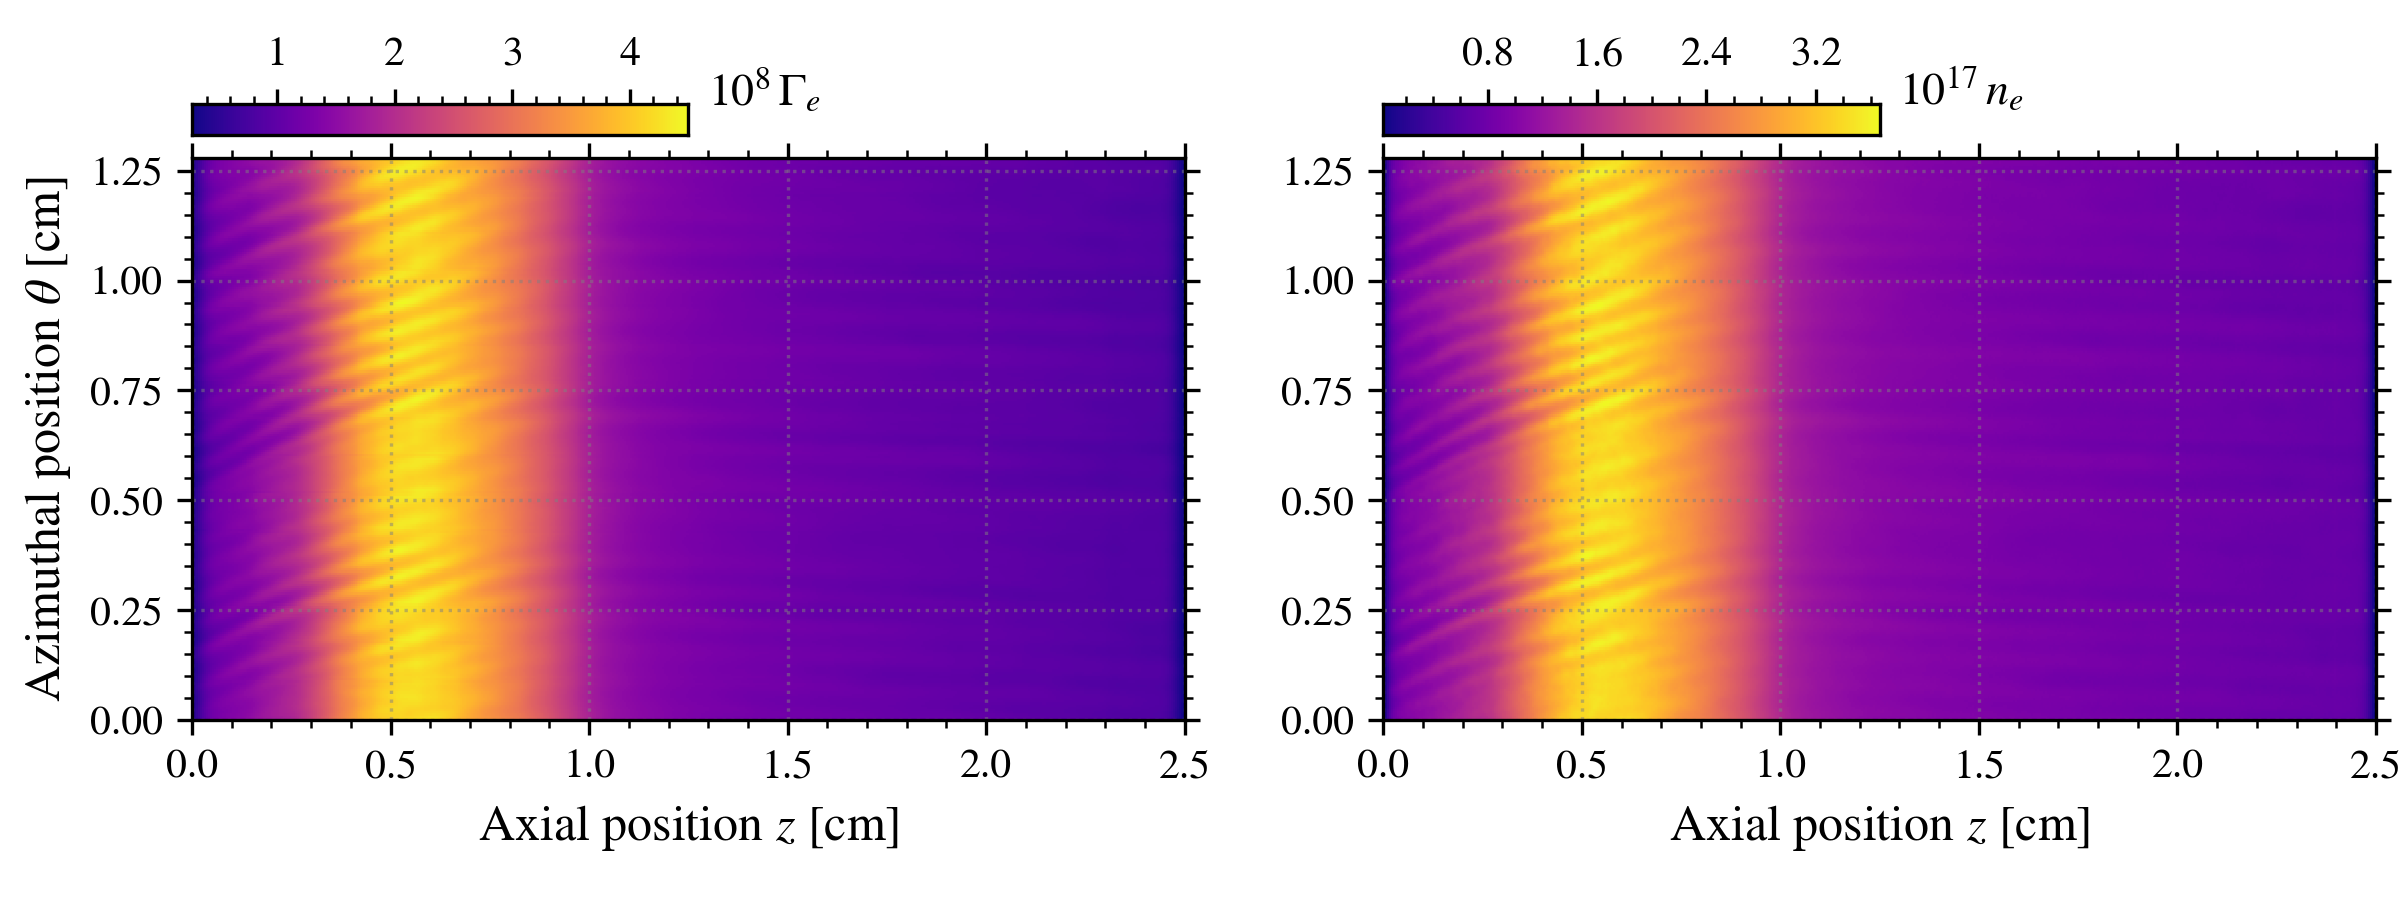
\includegraphics[width=\textwidth]{Flux_distribution}
    \caption{Axial-azimuthal distribution of the (left) electron flux at the wall and (right) the electron density, for the case $L_R=2\,\centi\meter$ at $t=10\,\micro\second$.}
    \label{fig-rfluxs}
  \end{figure}

  We see in \cref{fig-rfluxs}  that the radial flux presents the same spatial characteristics than that of the electron density, as expected from \cref{eq-Rlosses}
  This means that the loss of particle is greater at the maxima of the density oscillations.
  Under this condition, the amplitude of the oscillation will be directly reduced as 
  \[ \left. \deriv{\dne}{t} \right\rvert_{\Gamma_R} =  \gamma_R \dne \]
  with $\gamma_R < 0$ the damping rate of the instability due to the radial losses, which depends on the ion radial velocity $ \bar{v}_{i, r}$.
  To summarize, we have shown that this direct impact of the radial losses on the amplitude of the density fluctuation could result in a reduction of the instability amplitude, hence the wave energy $W$.
  
  \vspace{1em}
  The presence of a damping rate $\gamma_R$, combined with the reduction of the azimuthal drift velocity $u_{e, \theta}$ that is proportional to the instability growth rate, can explain the reduction of the wave amplitude at the steady-state.
  Indeed, the wave equation that takes into account the growth rate and the wave convection is \citep{martorelli2019}
  \begin{equation} \label{eq-wequation}
    \deriv{W}{t} + \div (\vect{u_i} W) = 2 \gamma_{\rm eff} W
  \end{equation}
  with $\gamma_{\rm eff}$ the effective growth rate, and $\vect{u_i} =u_{i, z} \vect{e_z}$  the ion mean velocity.
  As the radial losses do not affect significantly the axial electric field, $\vect{u_i}$ is the same for the three cases.
  Consequently, at steady state we have $\deriv{W}{t}=0$, so that if $\gamma_{\rm eff}$ is reduced because of $\gamma_R$, the wave energy $W$ is reduced as well.

  \FloatBarrier

\section{Spectral analyses of the waves} \label{subsec-fft}

  To better grasp the evolution of the instability with the radial losses, we proceed to a quantitative analysis of the instability by Fourier Transform.
  The spectral analyses are performed at $z_u=0.55\,\centi\meter$ for the upstream region, and $z_d=1.5\,\centi\meter$ for the downstream region.
  To give a better understanding of the wave observed, \Cref{fig-cut2D} shows the temporal evolution of the azimuthal electric field $E_{\theta}$  at the positions $z_u$ and $z_d$ when no radial losses are modeled.

  \begin{figure}[!hbt]
    \centering
    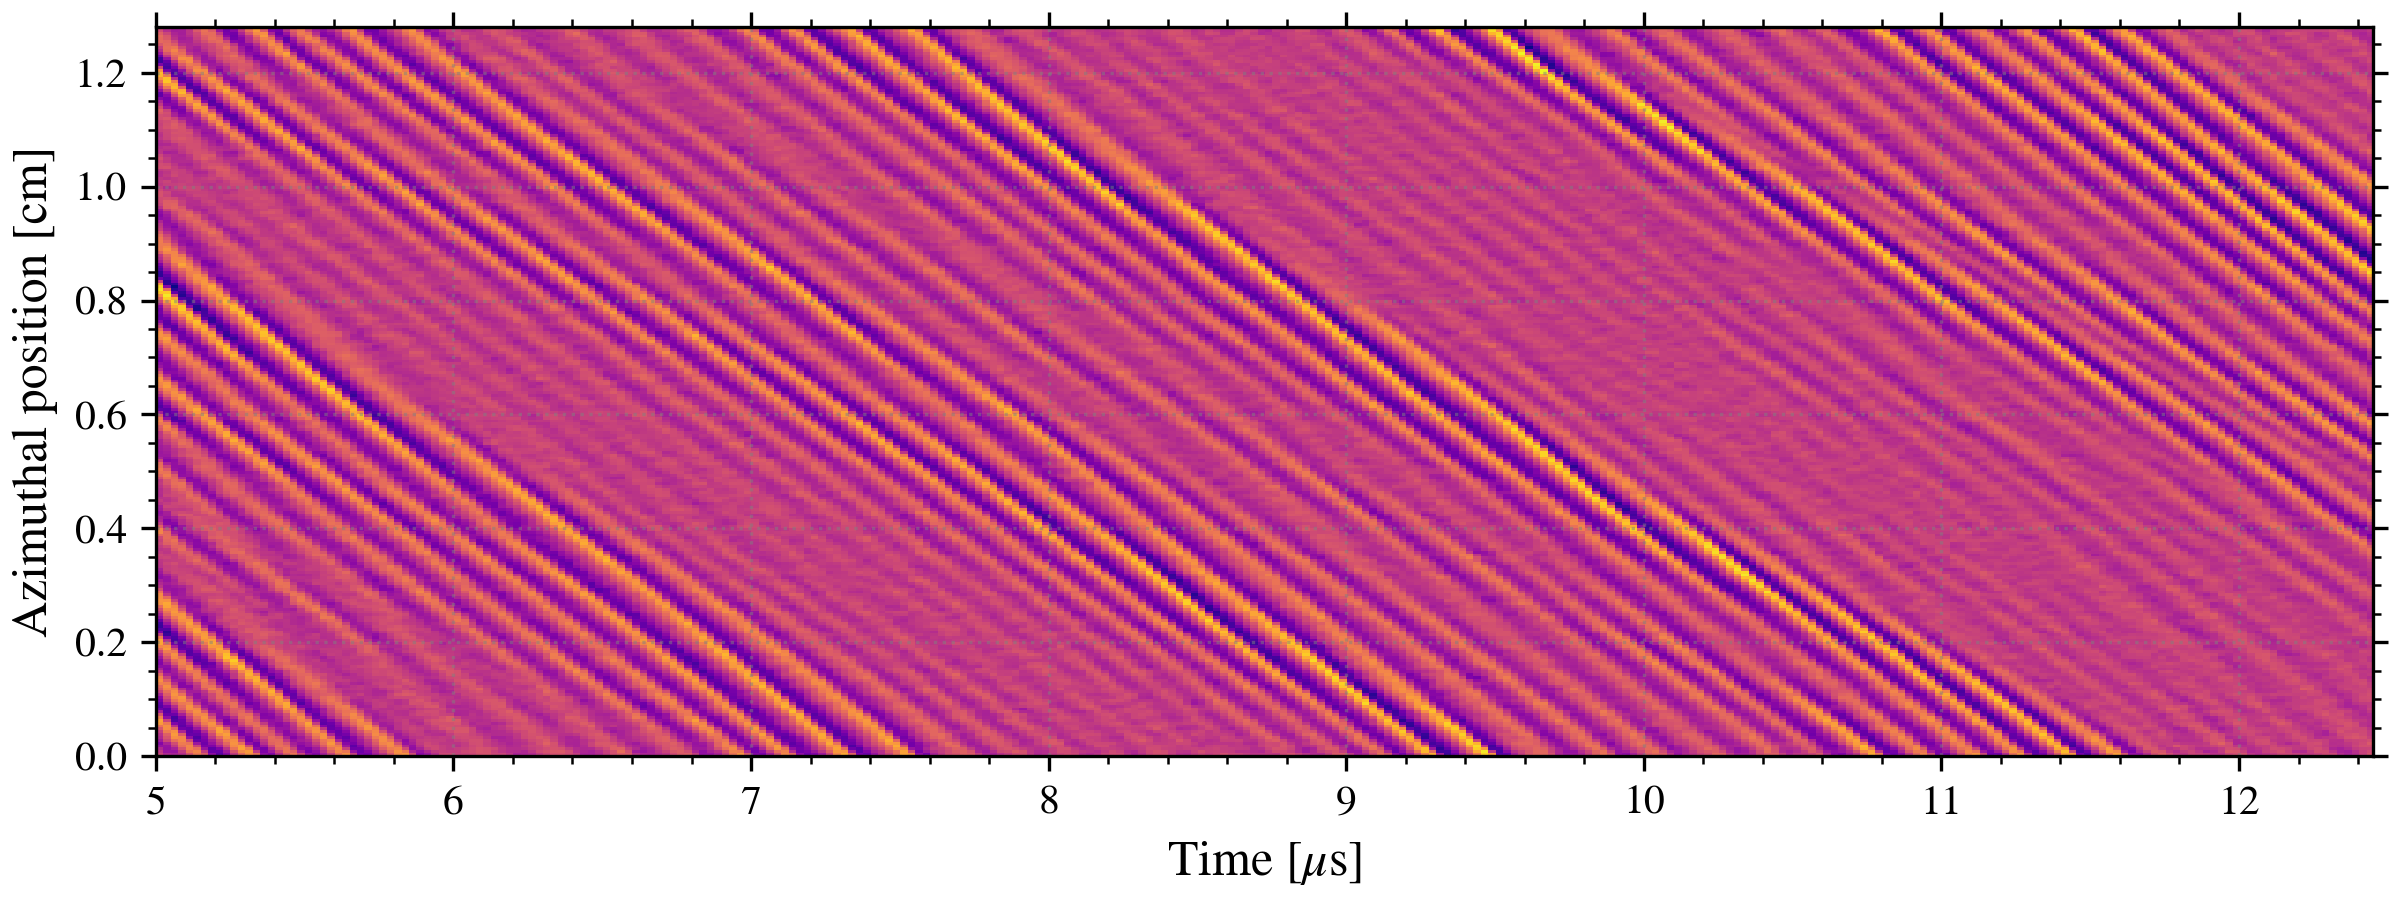
\includegraphics[width=0.8\textwidth]{Boeuf_noLr_y50_t200}
    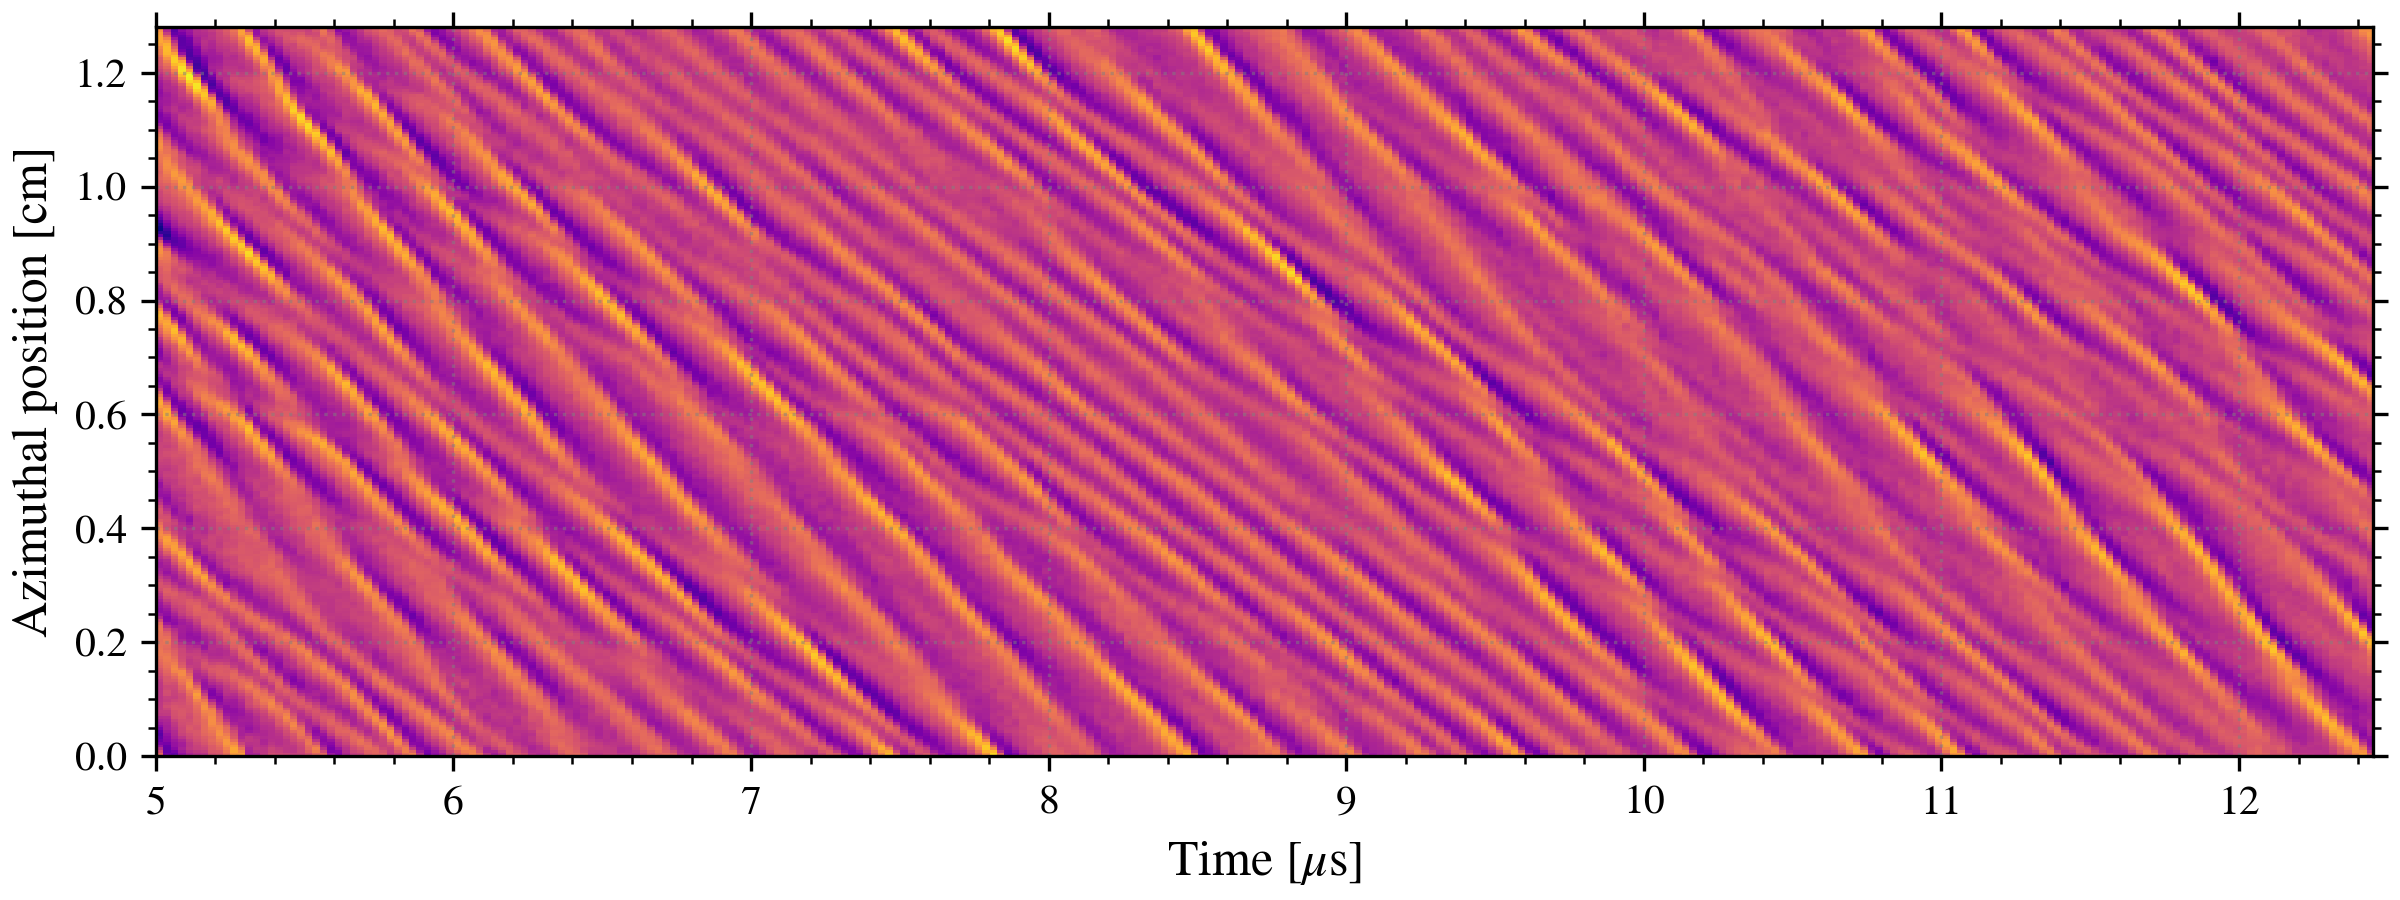
\includegraphics[width=0.8\textwidth]{Boeuf_noLr_y300_t200}
    \caption{Spatio-temporal evolution of the azimuthal electric field at (top) $z=z_u$ and (bottom) $z=z_d$ when no instability are present. The beginning of the simulation ($t<5\,\micro\second$) is not shown. }
    \label{fig-cut2D}
  \end{figure}


  For the upstream region, we see a monochromatic wave with a modulation of its amplitude.
  The downstream region is more complex, as there seems to be a combination of waves.
  We perform a \ac{2D} \ac{FFT} on the spatio-temporal azimuthal electric field to obtain the dispersion relation of the wave observed.
  \Cref{fig-fft2D_noLr_zu} shows the \ac{2D} \ac{FFT} obtained in ({\bf a}) the upstream region and ({\bf b}) the downstream region.
  We also display the \ac{1D} \ac{FFT} obtained by summing the \ac{2D} \ac{FFT} in one direction.
  Concerning the upstream region, we see that the waves follow one well-defined curve, which corresponds to the \ac{IAW} \ac{DR} \cref{eq-MIAW} using the local Debye length and ion plasma frequency.
  The maximum of the wave is located at $k_{\theta} = 8.5\,\radian\per\milli\meter$ and $\omega = 35\, \radian.\mega\hertz$.

  \begin{figure}[!hbt]
    \centering
    \begin{tabular}{@{} cc}
      \subfigure{Boeuf_noLr_FFT2D_y110_full}{a}{5,5} & 
      \subfigure{Boeuf_noLr_FFT2D_y300_full}{b}{5,5} \\
    \end{tabular}
    \caption{\acs{2D} and \acs{1D} \acs{FFT} of the azimuthal electric field in ({\bf a}) the upstream region $z=z_u$, and ({\bf b}) the downstream region at $z=z_d$, without radial losses. The black dotted lines highlight the position of the maximum of the \acs{2D} \acs{FFT}. The red dotted line corresponds the \acs{IAW} dispersion relation of \cref{eq-MIAW} at $z=z_u$, and the green dotted line the \acs{IAW} dispersion relation of \cref{eq-MIAW} at $z=z_d$.}
    \label{fig-fft2D_noLr_zu}
  \end{figure}

  The \ac{2D} \ac{FFT} in the downstream region is presented in \cref{fig-fft2D_noLr_zu}.{\bf b}.
  In contrast to the upstream region, we can see that the waves do not follow one well-defined curve.
  The wave characteristics of the upstream region can still be seen, but a larger and slower wave is overlaid to it.
  The maximum of the wave is located at $k_{\theta} = 3\,\radian\per\milli\meter$ and $\omega = 20\, \radian.\mega\hertz$.
  However, this new wave seems to follow the same dispersion relation as in the upstream region (green), instead of the \ac{DR} using the local plasma parameters (red).
  This could mean that the wave originates in the upstream region, and is convected to the downstream region without changing the wave \ac{DR}. 


  % \begin{figure}[hbt]
  %   \centering
  %   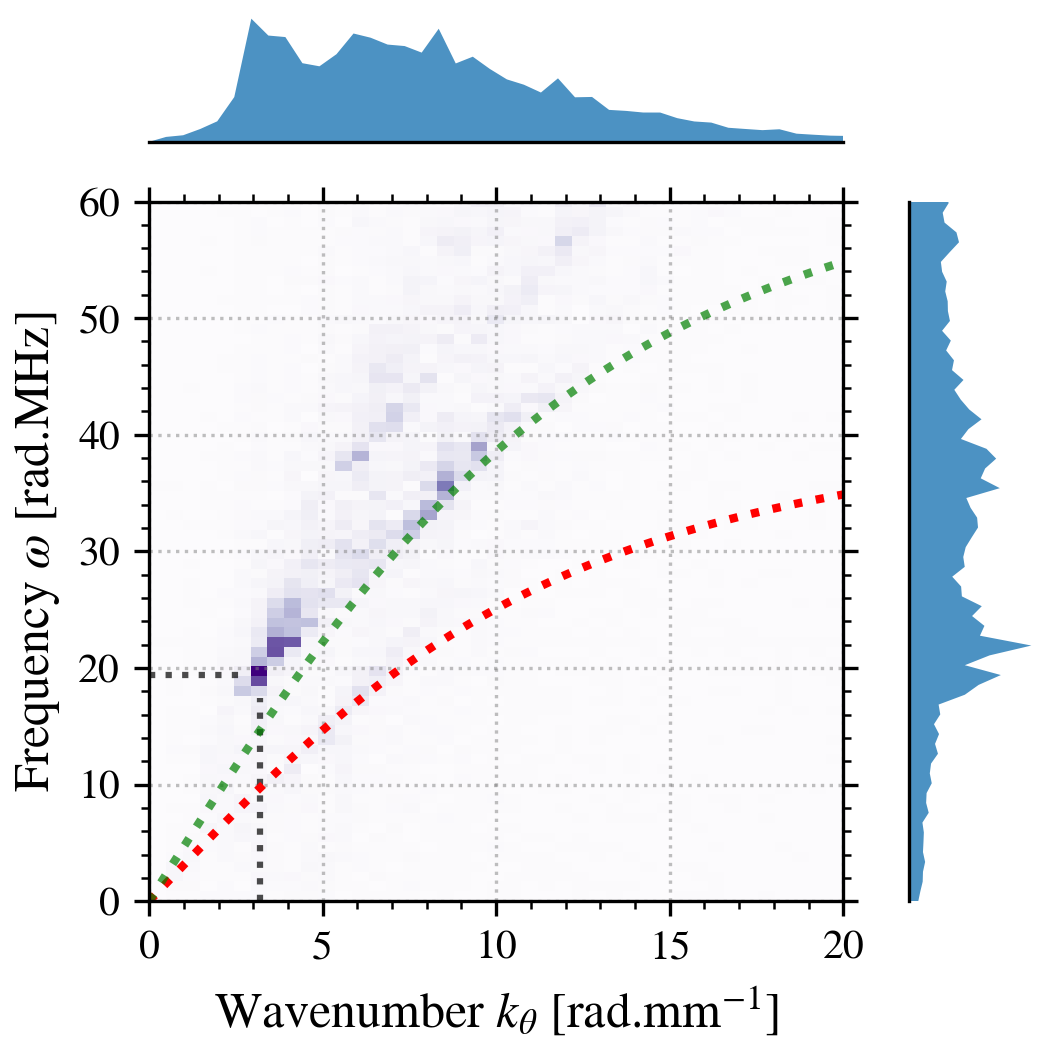
\includegraphics[width=5in]{Boeuf_noLr_FFT2D_y300_full}
  %   \caption{\acs{2D} and \acs{1D} \acs{FFT} of the azimuthal electric field in the downstream region $z=z_d$ without radial losses.  The black dotted lines highlight the position of the maximum of the \acs{2D} \acs{FFT}, and the red dashed line corresponds the \acs{IAW} dispersion relation of \cref{eq-MIAW}.}
  %   \label{fig-fft2D_noLr_zd}
  % \end{figure}


\subsection{Impact of the radial losses on the \acs{FFT}} \label{subsec-fft_losses}

  \Cref{fig-fft2D_Lr_zu,fig-fft2D_Lr_zd} show the \ac{2D} \ac{FFT} obtained with the radial losses in the upstream and downstream regions, respectively.
  In the upstream region, seen in \cref{fig-fft2D_Lr_zu}, the results are similar to the case without radial losses, as if the radial losses do not modify the nature of the wave.
  This comfort the qualitative analyze of \cref{subsec-azi_insta_Ztheta} that concluded that the algorithm used do not induce any numerical noise that creates unphysical results.


  \begin{figure}[!hbt]
    \centering
    \begin{tabular}{@{} cc}
      \subfigure{Boeuf_Lr4_FFT2D_y110_full}{a}{5,5} & 
      \subfigure{Boeuf_Lr2_FFT2D_y110_full}{b}{5,5} \\
    \end{tabular} 
    \caption{\acs{2D} and \acs{1D} \acs{FFT} of the azimuthal electric field in the upstream region $z=z_u$ with ({\bf a}) $L_R=4\,\centi\meter$, and ({\bf b}) $L_R=2\,\centi\meter$.  The black dotted lines highlight the position of the maximum of the \acs{2D} \acs{FFT}. The red dotted line corresponds  the \acs{IAW} dispersion relation of \cref{eq-MIAW} at $z=z_u$.}
    \label{fig-fft2D_Lr_zu}
  \end{figure}


  \begin{figure}[!hbt]
    \centering
    \begin{tabular}{@{} cc}
      \subfigure{Boeuf_Lr4_FFT2D_y300_full}{a}{5,5} & 
      \subfigure{Boeuf_Lr2_FFT2D_y300_full}{b}{5,5} \\
    \end{tabular}
    \caption{\acs{2D} and \acs{1D} \acs{FFT} of the azimuthal electric field in the downstream region $z=z_d$ with ({\bf a}) $L_R=4\,\centi\meter$, and ({\bf b}) $L_R=2\,\centi\meter$.  The black dotted lines highlight the position of the maximum of the \acs{2D} \acs{FFT}. The red dotted line corresponds the \acs{IAW} dispersion relation of \cref{eq-MIAW} at $z=z_u$, and the green dotted line the \acs{IAW} dispersion relation  of \cref{eq-MIAW} at $z=z_d$.}
    \label{fig-fft2D_Lr_zd}
  \end{figure}

  However, in the downstream region, showed in \cref{fig-fft2D_Lr_zd}, we do observe a difference due to the radial losses.
  For $L_R=4\,\centi\meter$, the low frequency-large wavelength wave already observed in the case without losses is present.
  Moreover, the waves remain slightly scattered in regard to the theoretical \ac{IAW} \ac{DR}.
  However, these two observations are less visible than without the radial losses.

  On the other hand, for $L_R=2\,\centi\meter$, both the low frequency wave and the scattering of the wave disappear.
  Only the waves observed in the upstream region remains.
  The evolution of the waves can also be seen in \Cref{fig-boeuf_fft_comparasion}, where the \ac{1D} spectra obtained in the downstream region for the three cases are overlaid.
  To compare the three cases, the wavenumber and the frequency are normalized by the Debye length $\lde$ and the ion plasma frequency $\opi$, respectively.
  Since we saw  in \cref{fig-fft2D_noLr_zu,fig-fft2D_Lr_zd} that the wave dispersion relation is better characterized by the upstream region, we use the values of $\lde$ and $\opi$ measured at $z=z_u$.


  \begin{figure}[hbtp]
    \centering
    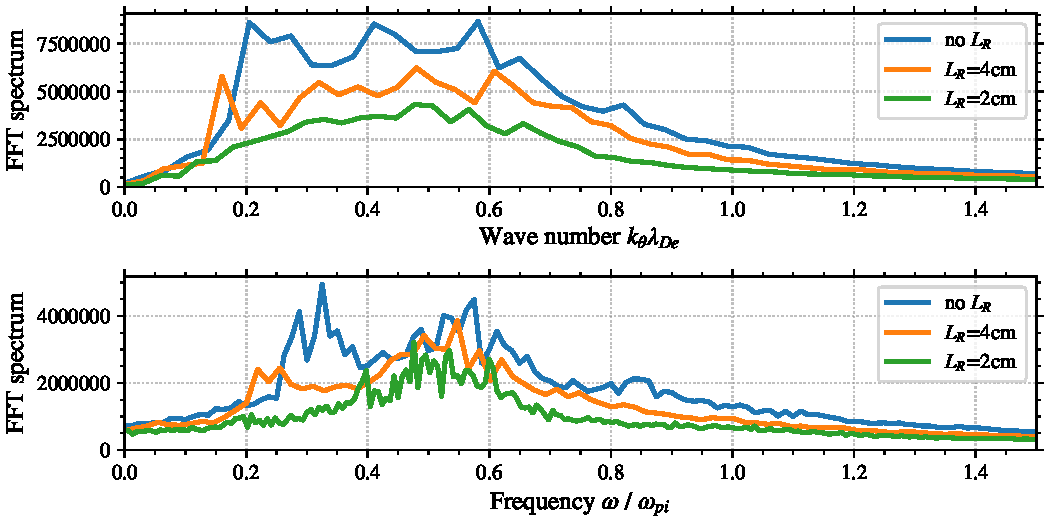
\includegraphics[width=0.9\textwidth]{Beuf_spectra_comp.pdf}
    \caption{Comparison of the frequency spectrum of the three axial-azimuthal simulations in the downstream region at $z=z_d$. On top, the spatial frequency spectra normalized by the Debye length $\lde$\string; bellow, the temporal frequency spectra normalized by the ion plasma frequency $\opi$. The values of $\lde$ and $\opi$ used are obtained in the upstream region at $z=z_u$, as the waves are better characterized by the upstream region.}
    \label{fig-boeuf_fft_comparasion}
  \end{figure}


  On the wavenumber spectrum, we see that the amplitudes of the waves are reduced by the radial losses, as previously observed in \cref{fig-snapshots}.
  We can also confirm that the difference on wavelength between the three cases comes from the evolution of the Debye length, as the three spectra are approximately centered around the same wavenumber.

  On the other hand, the temporal frequency spectra clearly show two maxima. 
  The first one can be seen around $\omega = 0.5 \opi$ for the three cases.
  The second is observed at lower frequencies\string: for the case without losses, it is clearly seen at  $\omega \simeq 0.3 \opi$\string; for the case $L_R=4\,\centi\meter$, the second maximum is closer to $\omega \simeq 0.25 \opi$\string; for the third case $L_R=2\,\centi\meter$, the second maximum disappear. %\footnote{We observe the small bump in the frequency spectrum at $\omega \simeq 0.2 \opi$, but it could simply be some noise. }
  
  \subsection{Axial evolution of the frequency spectra} \label{subsec-axialFFT}
  
  To finish with the analysis of the instability characteristics, we present in \cref{fig-axial_fft1D} the axial evolution of the \ac{1D} \ac{FFT} for the two extreme cases\string: without radial losses and with $L_R=2\,\centi\meter$.
  We can see in \cref{fig-axial_fft1D} that in the case without radial losses, the low frequency oscillation appears abruptly, close to $z=0.75\,\centi\meter$ which corresponds to the maximum of the magnetic field.
  On the contrary, it does not show up for $L_R=2\,\centi\meter$ in the frequency spectra.
  
 \begin{figure}[!hbt]
   \centering
   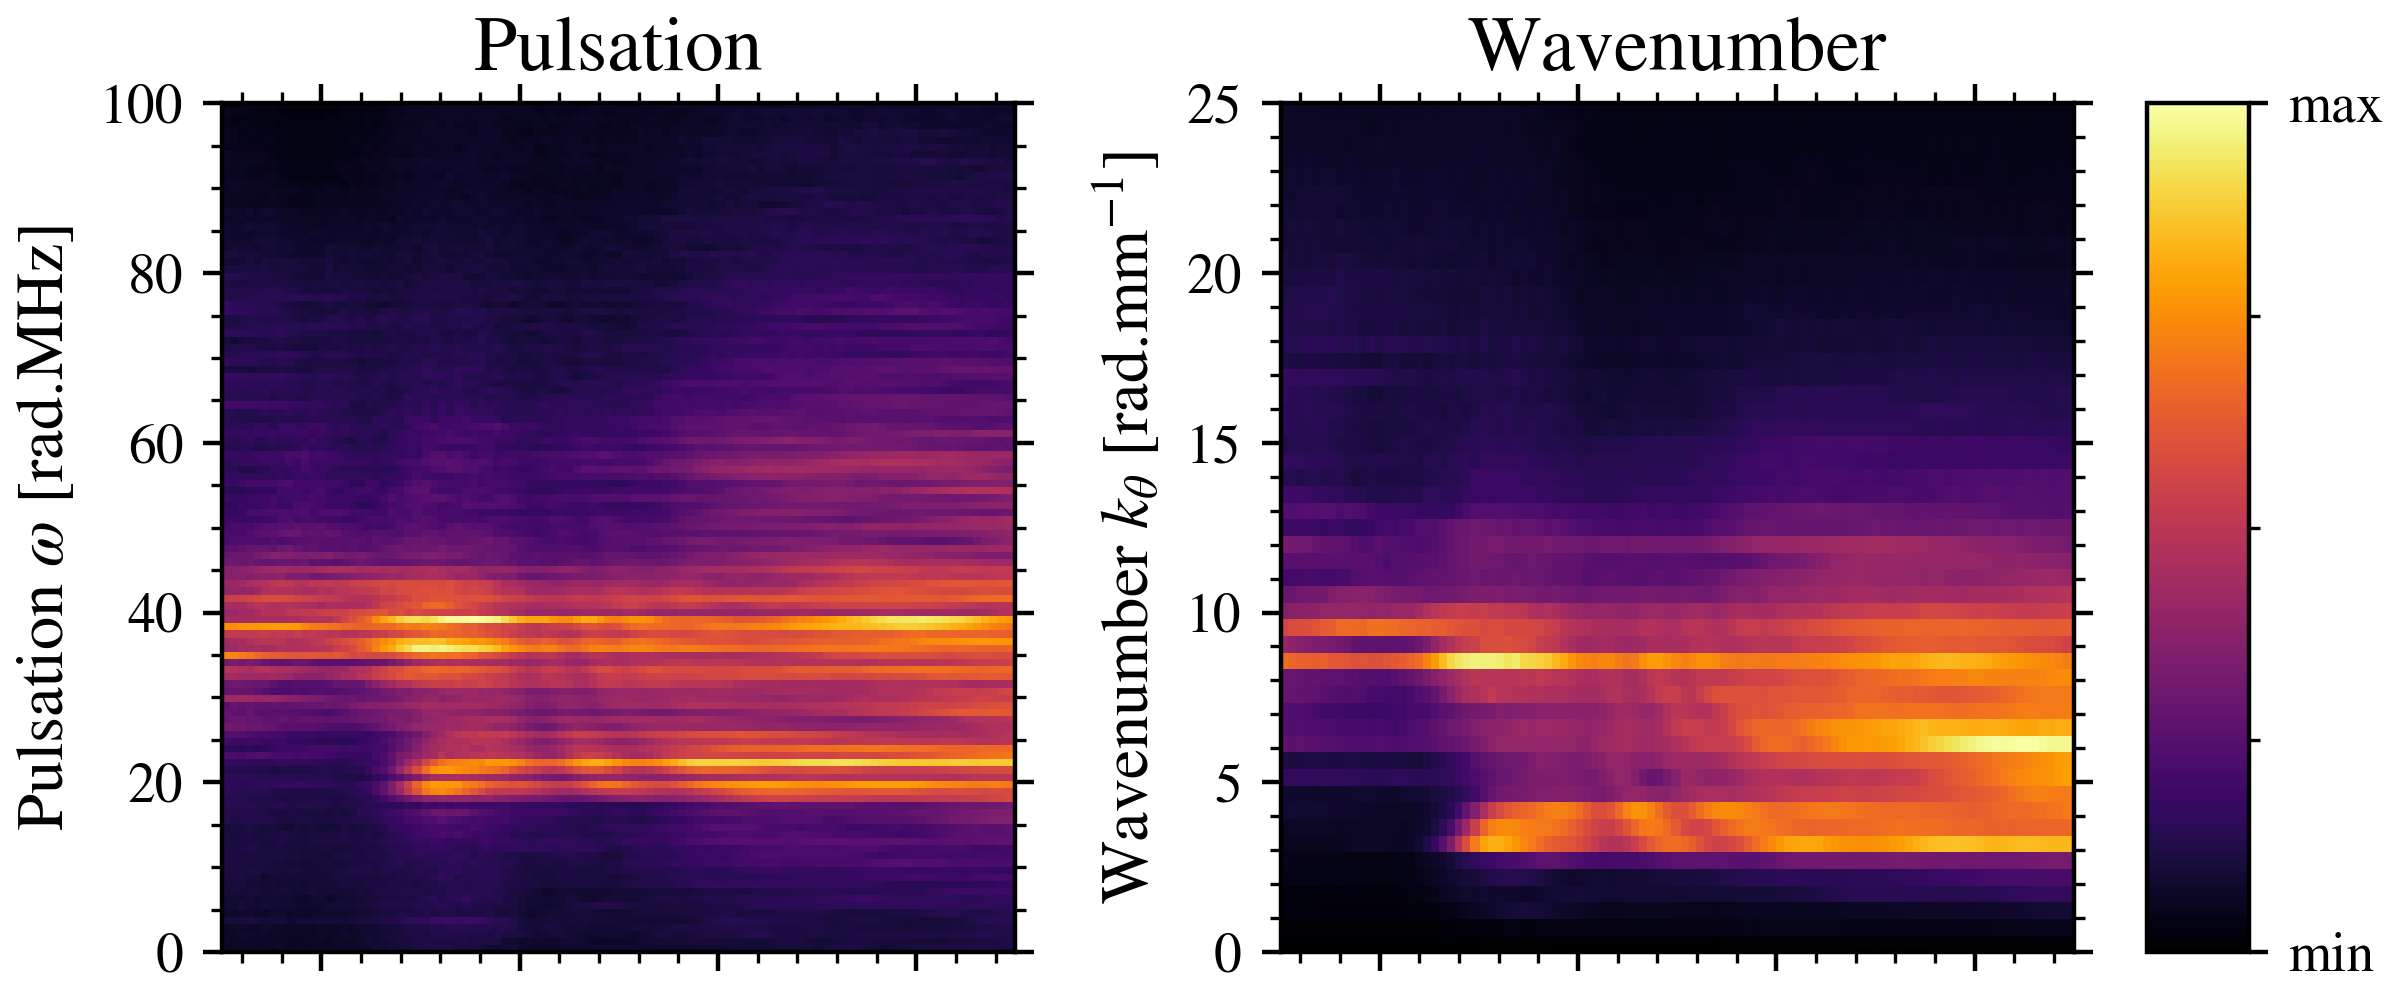
\includegraphics[width=\textwidth]{Boeuf_axila_evolution_fft1D_noLr}
   % 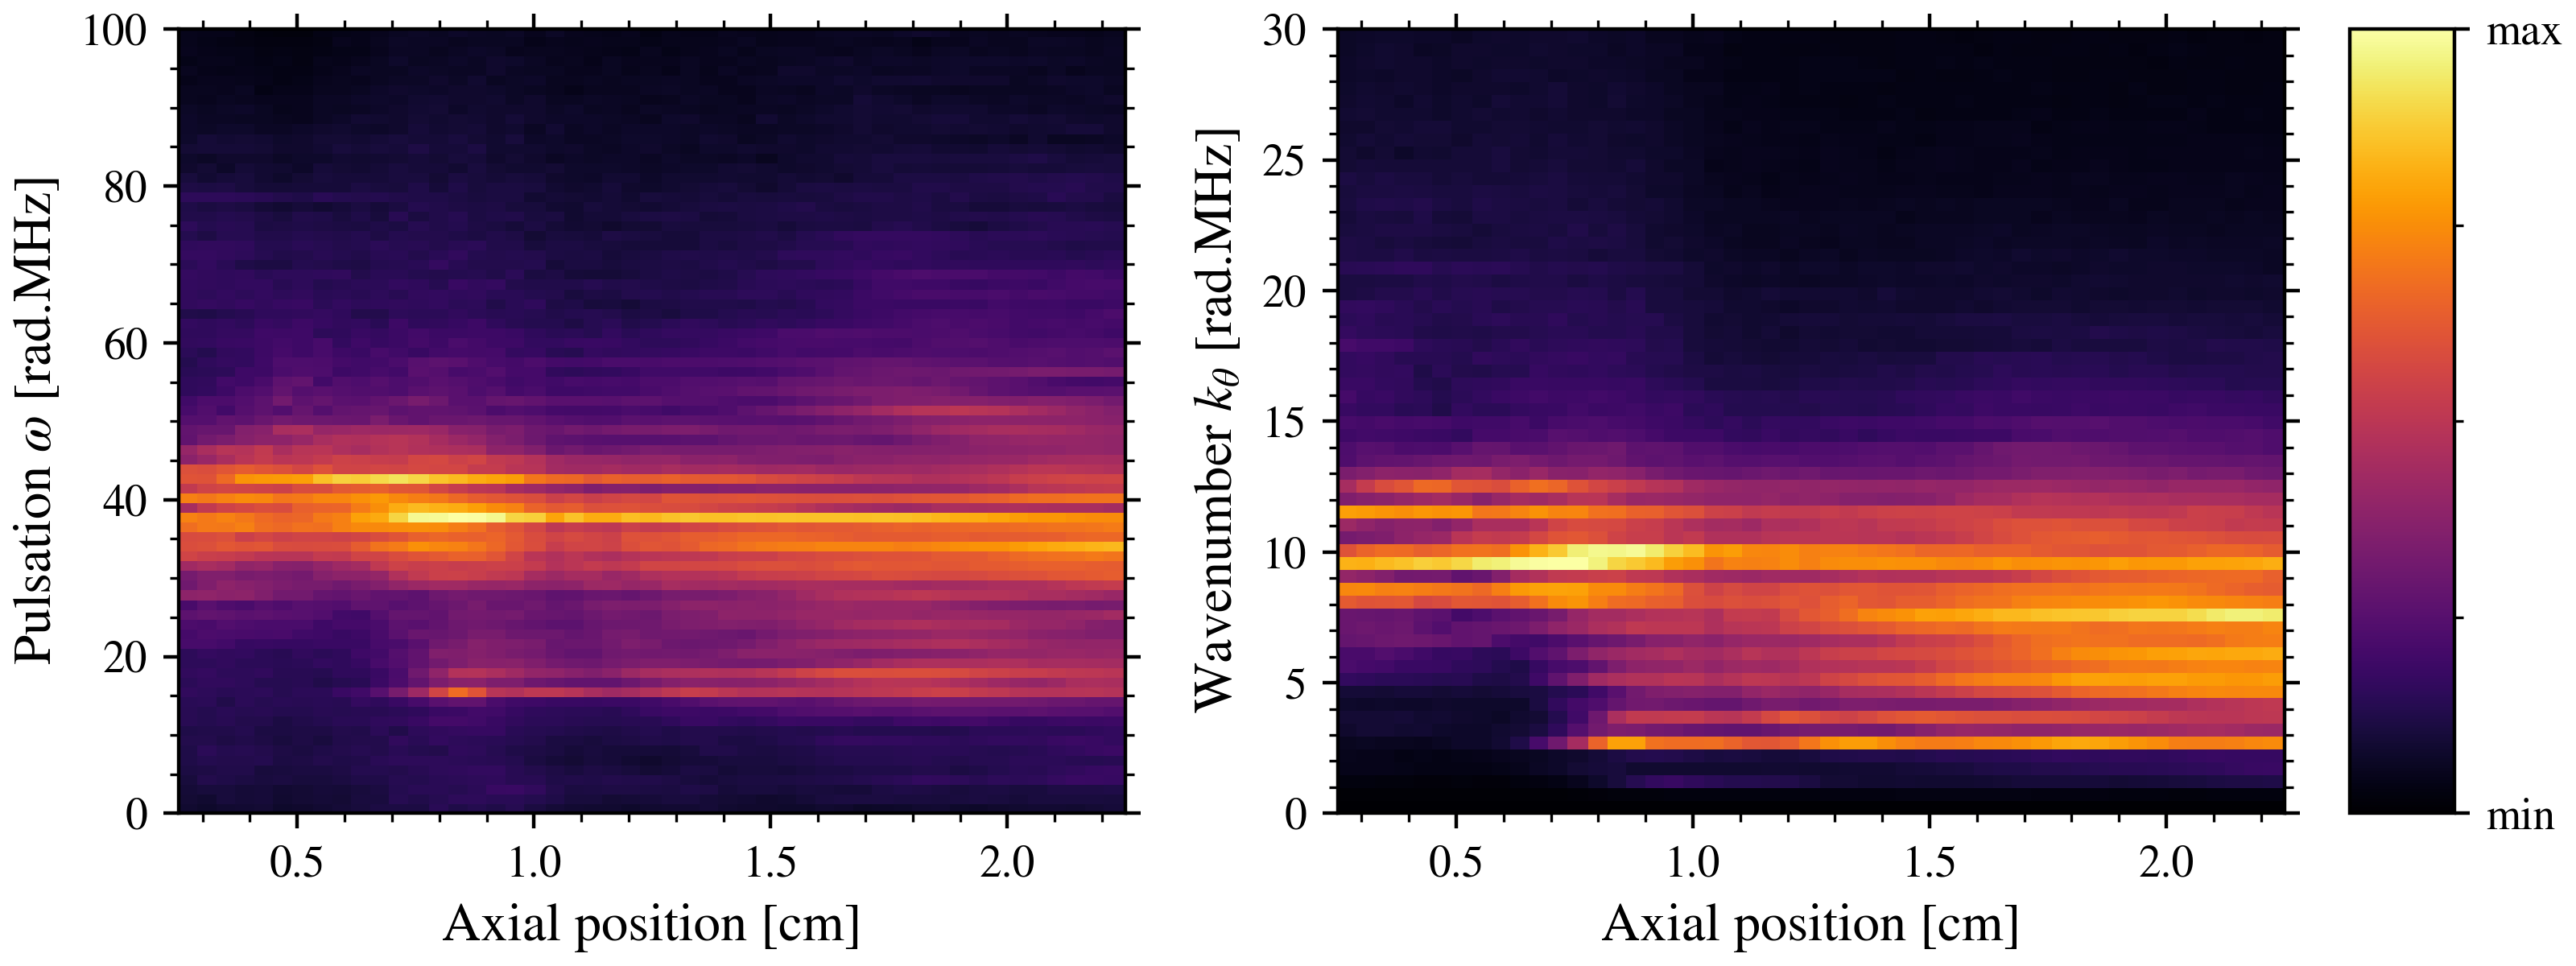
\includegraphics[width=\textwidth]{Boeuf_axila_evolution_fft1D_Lr4}
   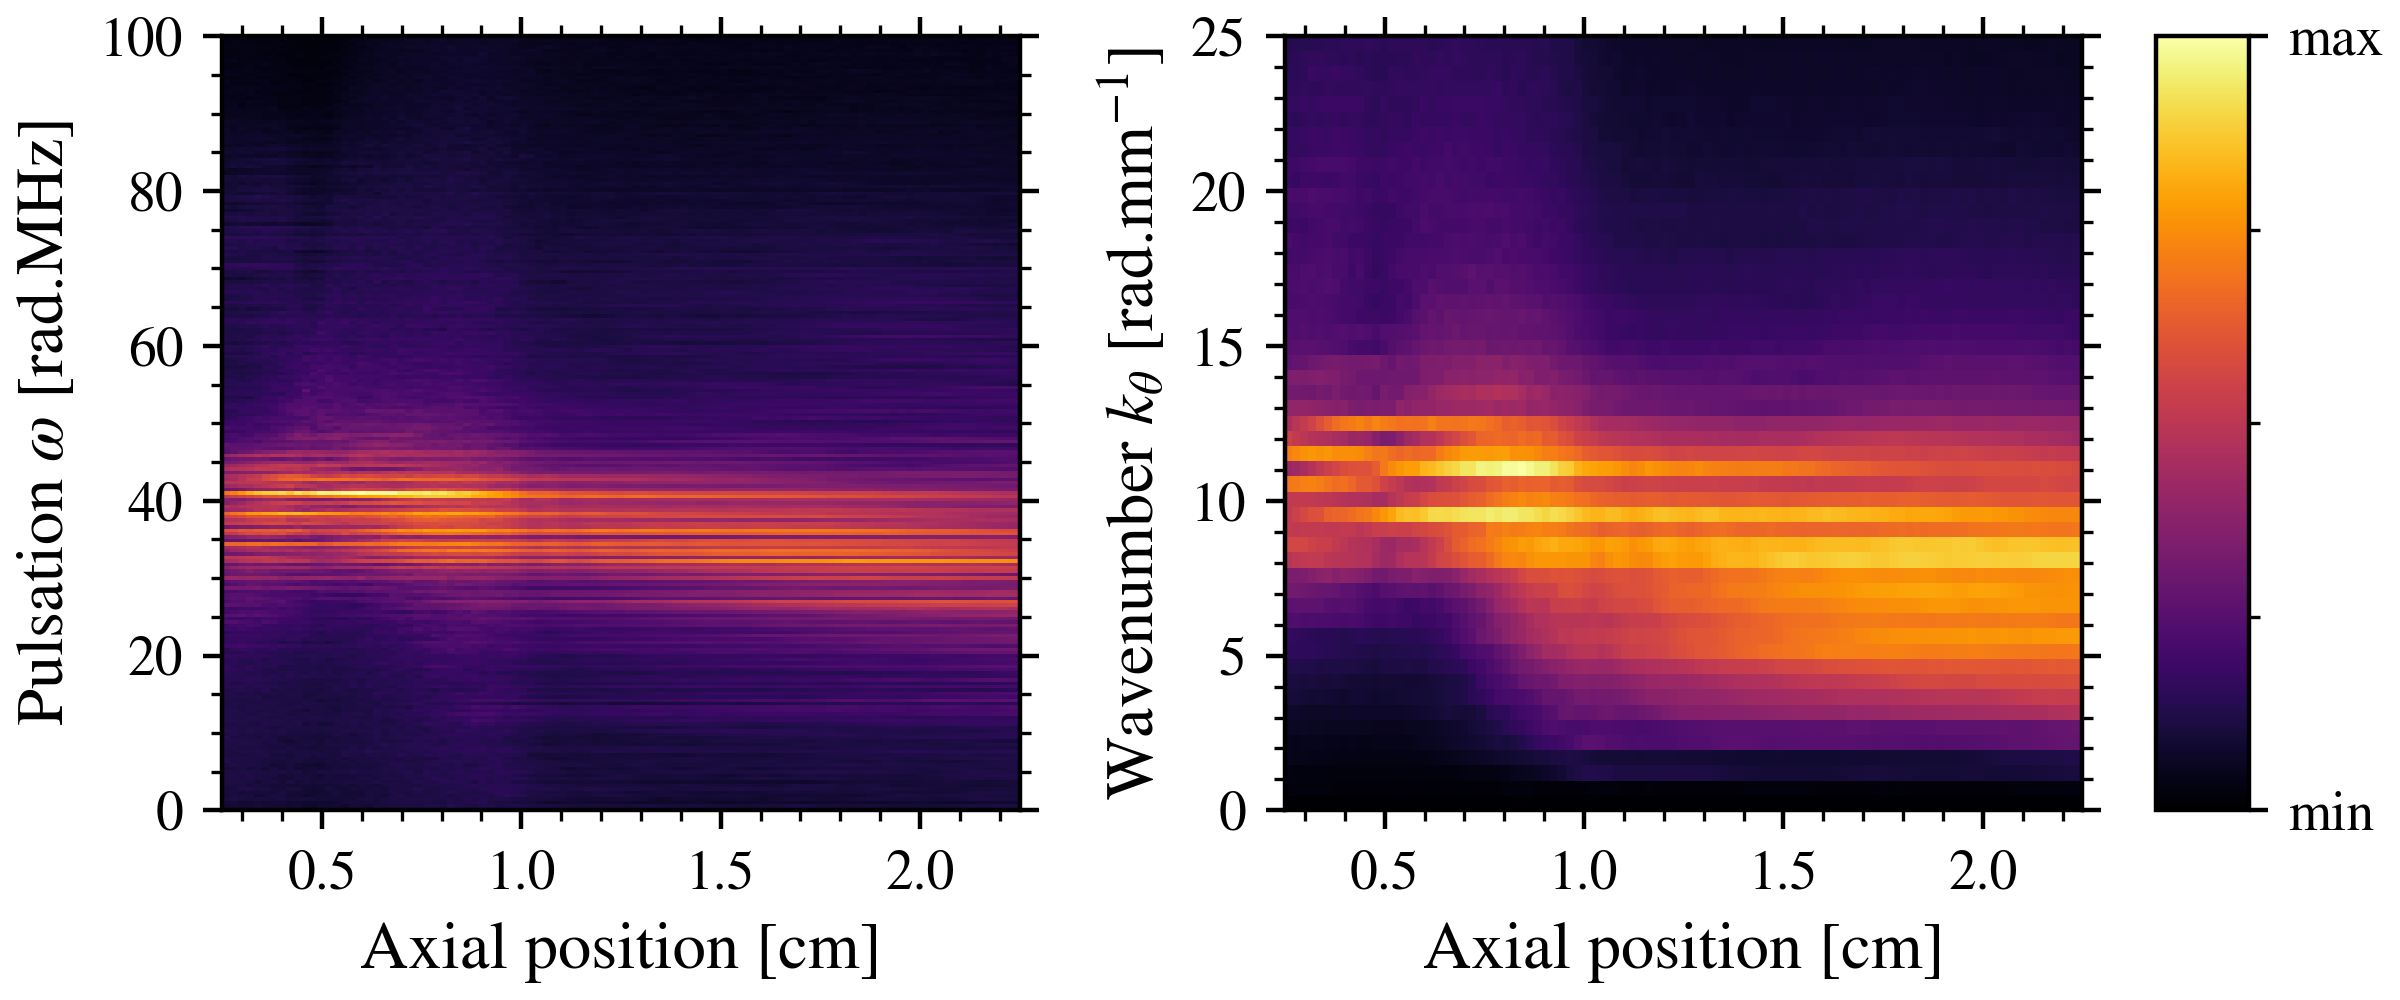
\includegraphics[width=\textwidth]{Boeuf_axila_evolution_fft1D_Lr2}
   \caption{Axial evolution of the \acs{1D} \acs{FT} on (left) the frequency and (right) the wavenumber for (top) no radial losses, and (bottom) $L_r=2\,\centi\meter$. }
   \label{fig-axial_fft1D}
 \end{figure}
  
  The low frequency oscillations seems to originate from a non-linear phenomena, such as an inverse cascade \citep{taccogna2019}.
  We have seen in \cref{sec-Ztheta-instability} that the effective growth rate is reduced by the radial losses, due to the reduction of $u_{e, \theta}$ and the presence of $\gamma_R$.
  However, the convection of the wave by the ions is not affected by the radial losses \citep{martorelli2019}.
  Consequently, we believe that due to the radial losses, the wave amplitude is smaller, and therefore does not reach the non-linear regime responsible of the low frequency large wavelength waves.

  % We have see previously that the \ac{1D} spectral aggregates the waves information, thus the larger wave cannot be directly observed by this way.
  % \Cref{fig-axial_maxwave_normalized} shows the axial evolution of the wave characteristics (pulsation and wavenumber) for the wave of maximum amplitude in the \ac{2D} \ac{FFT}, such as the one located by the dotted lines in \cref{fig-fft2D_noLr_zd}.
  % The pulsation $\omega$ is normalized by the local ion plasma pulsation $\opi$ given in \cref{fig-wpi_Lde}.
  % The azimuthal wavenumber $k_{\theta}$ is normalized by the local Debye length.
  % 
  % \begin{figure}[hbt]
  %   \centering
  %   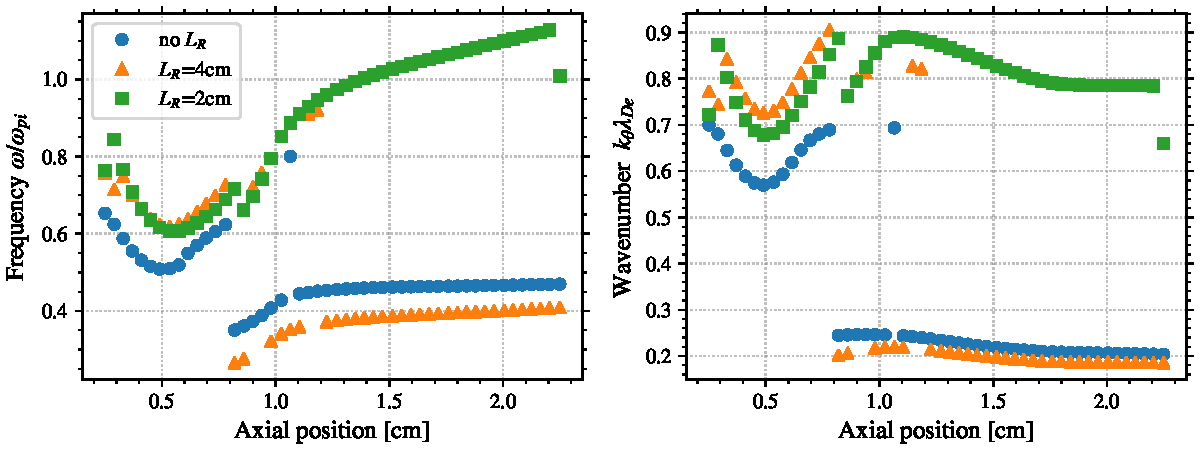
\includegraphics[width=\textwidth]{Boeuf_caracteristics_all_normalized}
  %   \caption{Axial evolution of (left) the frequency and (right) the wavenumber of the wave of maximum amplitude in the \acs{2D} \acs{FFT} for the three cases using the model of Boeuf. The pulsation and the wavenumber are normalized by the local ion plasma pulsation, respectively the Debye length.}
  %   \label{fig-axial_maxwave_normalized}
  % \end{figure}
  % 
  % We can see in \cref{fig-axial_maxwave_normalized} that the in the upstream region, the cases with radial losses ($L_R=2$ and $4\,\centi\meter$) present similar waves characteristics, with higher frequency and wavenumber than the case without radial losses.
  % However, in the downstream region the wave of maximum amplitude is the low frequency wave for both cases without losses and with $L_r=4\,\centi\meter$.
  % On the other hand, the case $L_R=2\,\centi\meter$ shows a small discontinuity, but the wave characteristics are very close to the wave in the upstream region.

\FloatBarrier
